\documentclass[12pt]{article}
\usepackage[a4paper, total={5.7in, 9in}]{geometry}
\usepackage{url}
\usepackage{hyperref}
\usepackage{graphicx}
\usepackage{booktabs}
\usepackage{amsmath}
\usepackage{listings}
\usepackage{xcolor}
\usepackage{soul}
\usepackage{tikz}
\usetikzlibrary{shapes, arrows.meta, positioning, fit}

\lstset{
  basicstyle=\ttfamily\small,
  breaklines=true,
  frame=single,
  backgroundcolor=\color{gray!10},
  keywordstyle=\color{blue},
  commentstyle=\color{green!50!black},
  stringstyle=\color{red!70!black},
  showstringspaces=false
}

\begin{document}
\title{BDI Multi-Agent System for Lung Nodule Evidence Extraction from Chest X-ray Reports}
\author{Sepehr Khodadadi Hosseinabadi\\
{\em 6660699@studenti.unige.it}\\
\url{https://github.com/sepehrkdi/lung_nodule_mas}}
\maketitle

% =============================================================================
% PROPOSAL PAGE (not counted)
% =============================================================================
\section{Details of the Proposal}
\label{sec:yourProposal}

\subsection{Full Specification of the Proposal}
\label{subsec:specification}

I will build a complete BDI multi-agent system in which all agents are BDI agents that interoperate by message passing, while only the CV agents use a pre-trained model and the NLP agents are fully implemented by me. The use case is lung nodule evidence extraction from chest X-ray radiology reports, paired with the corresponding X-ray images from the IU/Open-I chest X-ray collection (English reports). The dataset contains around 7,470 images and reports. I will use an NLP-based pre-filter to select 500 image--report pairs and automatically derive binary ground-truth labels (benign/malignant) from the report text for evaluation of the multi-agent consensus and NLP extraction outputs (entities + attributes + negation/uncertainty).



\subsection{The Kind of the Proposal}
\label{subsec:kind}

My proposal consists of a \textbf{creative project}.

\subsection{The Range of Points/Difficulty of the Proposal}
\label{subsec:points}

The degree of difficulty for this project is \textbf{hard}.

\pagebreak

% =============================================================================
% INTRODUCTION
% =============================================================================
\section{Introduction}
\label{sec:intro}

Lung cancer is the leading cause of cancer-related death worldwide, and early detection of pulmonary nodules is critical for improving patient outcomes. Radiology reports offer a rich source of structured and unstructured clinical information, yet extracting actionable evidence from free-text\footnote{free-text reports are reports that are not structured in a way that can be easily processed by a computer} reports remains a challenging NLP task. Simultaneously, medical imaging with deep learning has made progress in automated nodule detection, but individual models vary in their sensitivity and specificity.

This project addresses the problem of \emph{lung nodule evidence extraction and fusion} by combining three complementary AI paradigms within a multi-agent architecture:

\begin{enumerate}
    \item \textbf{Natural Language Processing (NLP):} Extracting structured nodule attributes (size, location, texture, descriptors), detecting mentions\footnote{mentions are the specific instances of nodule attributes mentioned in the report}, and determining negation/uncertainty status from free-text radiology reports.
    \item \textbf{Computer Vision (CV):} Obtaining nodule suspicion scores from chest X-ray images using the \texttt{TorchXRayVision} library~\cite{cohen2022xrv}, leveraging models pretrained on massive chest X-ray datasets.
    \item \textbf{Symbolic Reasoning:} Combining the outputs of multiple NLP and CV agents using first-order logic rules encoded in Prolog, \hl{implementing weighted consensus}, conflict detection, and binary classification (0=benign, 1=malignant) with supplementary clinical recommendations.
\end{enumerate}

The system is organized as a \emph{Belief--Desire--Intention (BDI) multi-agent system}~\cite{rao2005bdi}, adapted specifically for the Lung-Nodule MAS. In this context, \textbf{Beliefs} represent the specific diagnostic evidence held by an agent (e.g., a Radiologist believing a nodule is present with probability $p$, or a Pathologist believing a finding is negated). \textbf{Desires} represent the clinical objective to process a specific patient case (e.g., the goal \texttt{!analyze\_case}). \textbf{Intentions} are the runtime execution of image analysis models or NLP pipelines chosen to fulfill those goals. This architecture is appropriate for medical decision support because it mirrors the clinical workflow: independent specialists (radiologists, pathologists) generate findings that are synthesized by a coordinating physician (oncologist) into a final recommendation.

\subsection{Clinical Motivation}
\label{subsec:clinical-motivation}

In standard clinical practice for oncology patients, including those with lung malignancies, care is coordinated through multidisciplinary team (MDT) frameworks in which specialists such as radiologists, pathologists, surgeons, and oncologists collectively review imaging and clinical information to formulate diagnosis and management plans~\cite{pillay2016mdt}. Direct communication between radiologists and pathologists is uncommon in routine practice because they work independently and send reports to the treating physician. This clinically accurate architecture is reflected in my system design, where all agents report to the central Oncologist agent rather than communicating peer-to-peer.

\subsection{Dataset and Pre-processing}
\label{subsec:dataset}

The system operates on the IU/Open-I Indiana University Chest X-ray Collection~\cite{demsar2005openi}, which contains approximately 7,470 chest X-ray images (totaling $\sim$10\,GB) paired with free-text radiology reports. Detailed instructions for downloading and setting up this dataset are provided in the project's \href{https://github.com/sepehrkdi/lung_nodule_mas?tab=readme-ov-file#dataset}{\texttt{README.md}} file. This subset size is consistent with prior clinical NLP validation studies. For instance, Chapman et al.\ evaluated the NegEx negation-detection algorithm against a set of 1000 sentences containing 1235 clinical findings and diseases extracted from discharge summaries~\cite{chapman2001negex}. To focus the evaluation on cases where the NLP agents can perform meaningful extraction, I implemented a multi-stage pre-filter pipeline that combines XML metadata analysis with a composite NLP-richness scoring function:

\begin{enumerate}
    \item \textbf{Ingestion and MeSH\footnote{Medical Subject Headings} Parsing:} The \href{https://github.com/sepehrkdi/lung_nodule_mas/blob/main/data/nlmcxr_loader.py}{\texttt{NLMCXR\_Loader}} scans all XML report files. In addition to extracting the standard report sections (\texttt{FINDINGS}, \texttt{IMPRESSION}, \texttt{INDICATION}, \texttt{COMPARISON}), the parser now extracts \texttt{<MeSH>} annotations from each XML file. These include \texttt{<major>} tags (expert-assigned indexing terms such as ``Opacity/lung/upper lobe/right'' or ``normal'') and \texttt{<automatic>} tags (machine-generated terms). MeSH annotations provide structured metadata about the clinical content of each case without requiring full NLP processing.
    \item \textbf{NLP Richness Scoring:} Each case is scored on six binary criteria (each worth 1 point, yielding a score in $[0, 6]$):
    \begin{enumerate}
        \item \emph{Text length:} combined \texttt{FINDINGS} + \texttt{IMPRESSION} contains $\geq 80$ characters. Empirical analysis of the dataset indicates that reports below this threshold (approximately the bottom 3\%) are typically ``normal'' templates lacking specific findings, whereas reports above this length contain extractable pathological entities.
        \item \emph{Non-normal MeSH:} at least one \texttt{<major>} tag that is not just ``normal'', leveraging the expert indexing provided with the collection~\cite{demsar2005openi}.
        \item \emph{Target entity present:} regex match finds a clinical entity (nodule, mass, opacity, consolidation, etc.).
        \item \emph{Entity not fully negated:} at least one entity is \emph{not} linguistically negated, ensuring the report contains positive evidence~\cite{chapman2001negex, peng2018negbio}.
        \item \emph{Both sections non-empty:} \texttt{FINDINGS} and \texttt{IMPRESSION} both contain text.
        \item \emph{Anatomical location specified:} a laterality + anatomy pattern is present (e.g., ``right upper lobe'', ``left lung base'').
    \end{enumerate}
    \item \textbf{Ground-Truth Derivation:} Each case is independently passed through the NLP-based ground-truth extractor (Section~\ref{subsec:groundtruth}), which utilizes \emph{only the IMPRESSION section} to assign a binary label: 1 (malignant) or 0 (benign). This separation ensures the ground truth reflects the radiologist's synthesized diagnosis. Cases returning $-1$ (Indeterminate) are excluded.
    \item \textbf{Subset Selection:} Cases with richness score $\geq 3$ are retained and ranked in descending order of score. The top 500 cases are selected to form the \emph{Evaluation Subset}. In my dataset, 2{,}898 of 3{,}955 cases score $\geq 3$, providing candidates; 420 cases achieve the maximum score of 6.
\end{enumerate}

Table~\ref{tab:richness-dist} shows the score distribution across the full dataset.

\begin{table}[h]
\centering
\begin{tabular}{ccccccc}
\toprule
\textbf{Score} & 0 & 1 & 2 & 3 & 4 & 5--6 \\
\midrule
\textbf{Cases} & 84 & 92 & 793 & 1{,}210 & 770 & 1{,}006 \\
\bottomrule
\end{tabular}
\caption{Distribution of NLP richness scores across all 3{,}955 NLMCXR cases. Cases with score $\geq 3$ (77\%) are eligible for the Evaluation Subset.}
\label{tab:richness-dist}
\end{table}

This richness-based filtering ensures that the selected cases contain sufficient textual content for the Pathologist agents' regex, NER, and negation-detection pipelines to operate on, rather than relying solely on binary keyword presence.

\subsection{Ground Truth Definition}
\label{subsec:groundtruth}

For the entire dataset, a binary label (1=malignant, 0=benign) is automatically derived from the \texttt{IMPRESSION} section of the original radiology reports. The \texttt{IMPRESSION} section represents the radiologist's final diagnosis and synthesis. A case is labeled ``malignant'' (1) if this section contains un-negated suspicious keywords (``suspicious'', ``malignant'', ``ill-defined'', ``spiculated''), otherwise ``benign'' (0).

Using NLP-derived labels as ground truth commonly termed a ``Silver Standard'' is an established practice in large-scale medical imaging research where manual annotation at scale is infeasible. Two landmark datasets adopt this approach: CheXpert~\cite{irvin2019chexpert} applies a rule-based NLP labeler (mention extraction $\rightarrow$ negation/uncertainty classification $\rightarrow$ label aggregation) to assign 14 observation labels from radiology reports, while MIMIC-CXR-JPG~\cite{johnson2019mimiccxr} reuses the same CheXpert labeler to produce labels for over 370{,}000 chest radiographs. Both projects demonstrate that carefully designed rule-based NLP pipelines produce labels of sufficient quality for training and evaluating deep learning systems at scale.

My ground-truth extraction pipeline follows the same architectural pattern as the CheXpert labeler:
\begin{enumerate}
    \item \emph{Mention extraction}: keyword and regex patterns identify clinical entities (nodule, mass, opacity, spiculated, etc.);
    \item \emph{Negation and uncertainty detection}: NegEx-style~\cite{chapman2001negex} rules classify whether entities are affirmed, negated, or uncertain (cf.\ NegBio~\cite{peng2018negbio});
    \item \emph{Label aggregation}: the final binary label is derived from the presence of un-negated suspicious keywords.
\end{enumerate}
The key difference is scope: while CheXpert labels 14 observations, my extractor targets a single binary decision (benign vs.\ malignant) optimized for lung nodule assessment.

Naturally, the NLP agents (Section~\ref{subsubsec:pathologists}) are restricted to analyzing only the \texttt{FINDINGS} section, which contains the raw clinical observations. This separation prevents ``circular confirmation'' where agents purely re-read the diagnosis they are supposed to infer. Note that neither CheXpert nor MIMIC-CXR enforce this separation---both apply their labeler to the full report text. My approach is therefore more conservative: the agents must \emph{infer} the diagnosis from observations, while the ground truth is derived from the radiologist's explicit synthesis.

\subsection{Contributions}
\label{subsec:contributions}

The main contributions of this project are:

\begin{enumerate}
    \item A BDI multi-agent system with \textbf{7 agent instances} across 3 agent types, communicating via FIPA-ACL message passing.
    \item An evaluation methodology where NLP agents must infer a diagnosis from observational data (\texttt{FINDINGS}) while being evaluated against the radiologist's explicit diagnosis (\texttt{IMPRESSION}).
    \item A custom NLP pipeline for lung nodule evidence extraction implementing: report section splitting with section weighting, entity and attribute extraction, measurement normalization, and NegEx-style negation and uncertainty detection.
    \item A dependency-anchored frame building module that utilizes grammatical structure to strictly associate attributes (size, location, texture) with the correct nodule entity, resolving the ``bag-of-words'' problem in complex multi-nodule reports.
    \item A Prolog-based consensus mechanism that performs weighted voting, disagreement detection, conflict resolution, and binary classification (benign vs.\ malignant) with explanation generation.
    \item A dynamic, per-case weight assignment mechanism that adjusts agent reliability weights based on the information richness of the available radiology images and pathology reports, replacing static hardcoded weights.
    \item A multi-factor NLP-richness scoring function that combines MeSH metadata, entity detection, negation awareness, and structural completeness to select evaluation cases where the NLP agents can perform meaningful extraction.
    \item An anatomically-calibrated size estimation method for the rule-based radiologist that uses blob detection with a chest X-ray field-of-view model, replacing a na\"ive pixel-dimension heuristic that produced clinically implausible values.
    \item Explicit handling of unknown measurements: agents return \texttt{None} with a provenance tag (\texttt{size\_source}) instead of hardcoded defaults, and the consensus engine reduces the weight of agents that could not determine nodule size.
    % \item Binary classification (0=benign, 1=malignant) with threshold=0.5, replacing the original 5-class Lung-RADS categorization. Lung-RADS categories and TNM staging are retained as supplementary clinical recommendations.
    \item An end-to-end evaluation on real clinical reports using NLP-derived binary ground truth for system-level classification.
\end{enumerate}


% =============================================================================
% BACKGROUND
% =============================================================================
\section{Background and Related Work}
\label{sec:background}

\subsection{NLP in Radiology}
\label{subsec:nlp-radiology}

Pons et al.~\cite{pons2016nlpradiology} present a systematic review of NLP applications in radiology, describing a complete pipeline consisting of: (i) report section splitting (e.g., separating Findings from Impression); (ii) tokenization and normalization (handling abbreviations and standardizing measurements); (iii) syntax and semantic processing; and (iv) application-specific extraction. Systems like CheXpert~\cite{irvin2019chexpert} and NegBio~\cite{peng2018negbio} have demonstrated that symbolic NLP can achieve high accuracy in this domain without the need for large annotated datasets required by deep learning models. They emphasize that \emph{negation detection} is essential for clinical NLP, since a large proportion of medical concepts in radiology reports appear in negated contexts (e.g., ``no evidence of nodule''). My NLP pipeline follows this structure, with each stage implemented across three specialized Pathologist agents.

\subsection{Negation and Uncertainty Detection}
\label{subsec:negation}

Chapman et al.~\cite{chapman2001negex} introduced NegEx, a simple algorithm for identifying negated findings in clinical text. The algorithm operates by: (1) detecting \emph{trigger phrases} (e.g., ``no'', ``without'', ``denies'', ``ruled out''); (2) defining a forward or backward \emph{scope window} (typically 5--6 words); and (3) marking any medical entity within that scope as negated. Harkema et al.~\cite{harkema2009context} extended this approach with ConText, adding support for experiencer identification and temporal status.

For uncertainty detection, the CheXpert labeler~\cite{irvin2019chexpert} demonstrated that rule-based approaches can effectively classify radiology report mentions as positive, negative, or uncertain using trigger words such as ``possible'', ``cannot exclude'', ``may represent'', and ``suggestive of''. While CheXpert targets 14 chest X-ray observations, my project applies the same principles to the narrower task of nodule-specific attribute extraction.

\subsection{BDI Multi-Agent Systems}
\label{subsec:bdi}

The Belief--Desire--Intention (BDI) architecture~\cite{rao2005bdi} models rational agents that maintain: \emph{beliefs} (information about the environment), \emph{desires} (goals to achieve), and \emph{intentions} (committed plans). This architecture is implemented using the SPADE-BDI framework~\cite{spadebdi2023}, which extends the SPADE middleware~\cite{palanca2020spade} to support AgentSpeak(L) plans. The use of AgentSpeak(L) for defining agent reasoning follows the standard approach for programming BDI agents popularized by Jason~\cite{bordini2007multi}. In my implementation, \href{https://github.com/sepehrkdi/lung_nodule_mas/blob/main/spade_main.py}{\texttt{spade\_main.py}} serves as the entry point, initializing specialized BDI agents that execute strict AgentSpeak logic defined in `.asl` files.

\subsection{Multi-Agent Consensus}
\label{subsec:consensus-bg}

Collective intelligence theory suggests that aggregating independent opinions often outperforms individual experts. Wolf et al.~\cite{wolf2015collective} demonstrated that pooling the decisions of multiple radiologists significantly improves diagnostic accuracy (both sensitivity and specificity). Similarly, calculating consensus from double reading is a standard quality assurance practice in radiology~\cite{schaefer2018double}. My system automates this ``double reading'' by using multiple agents (both CV and NLP) and resolving their conflicts via a structured voting mechanism.

\subsection{Neuro-Symbolic AI}
\label{subsec:neurosymbolic-bg}

Neuro-symbolic AI seeks to combine the learning capability of neural networks with the reasoning transparency of symbolic logic~\cite{garcez2019neurosymbolic}. In high-stakes domains like medicine, pure black-box models are often insufficient due to lack of explainability. Recent systems like ProCDS~\cite{tan2025procds} have shown that using Prolog to enforce logical consistency on top of statistical model outputs can reduce errors and provide clinically meaningful explanations. The current project also adopts precisely this neuro-symbolic approach: CNNs and NLP agents provide perception, while Prolog provides reasoning.

\subsection{Medical Decision Standards}
\label{subsec:medical-standards}

The Oncologist agent's reasoning layer encodes decision criteria grounded in two publicly documented medical standards:

\begin{itemize}
    \item \textbf{Lung-RADS v1.1}~\cite{acr2019lungrads}: The American College of Radiology's Lung Imaging Reporting and Data System defines categories from 1 (Negative) to 4X (Highly Suspicious) based on nodule size, texture, and morphological features. This provides a clear, codifiable mapping from nodule evidence to management recommendations.
    \item \textbf{TNM Staging (8th Edition)}~\cite{amin2017ajcc}: The AJCC TNM classification provides tumor staging based on tumor size (T), lymph node involvement (N), and distant metastasis (M). I reference the staging thresholds to ensure the rule base uses medically consistent vocabulary.
\end{itemize}


% =============================================================================
% SYSTEM ARCHITECTURE
% =============================================================================
\section{System Architecture}
\label{sec:architecture}

\subsection{Overview}
\label{subsec:arch-overview}

The system emulates the real-world clinical workflow in which independent specialists generate domain-specific reports that are subsequently integrated by a coordinating clinician to inform diagnosis and management:

\begin{figure}[ht]
\centering
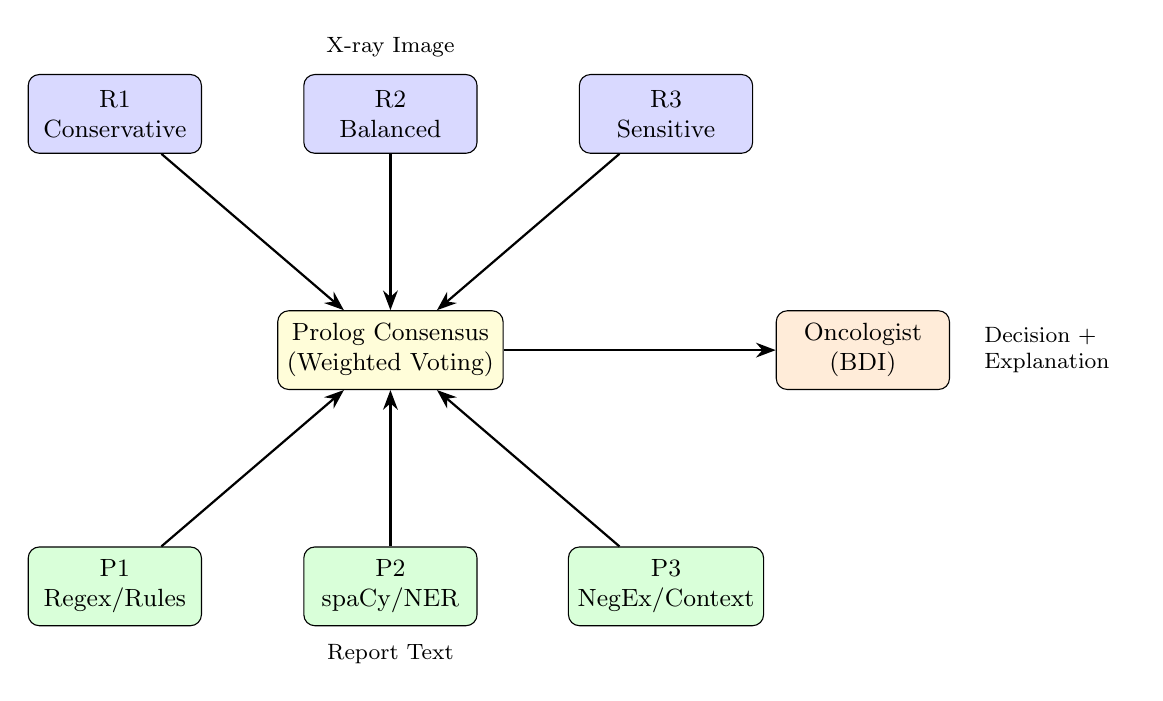
\begin{tikzpicture}[
    agent/.style={draw, rounded corners, minimum width=2.2cm, minimum height=1cm, align=center, font=\small},
    rads/.style={agent, fill=blue!15},
    paths/.style={agent, fill=green!15},
    onc/.style={agent, fill=orange!15},
    prolog/.style={agent, fill=yellow!15},
    arr/.style={-{Stealth[length=2.5mm]}, thick},
]
% Radiologists
\node[rads] (r1) at (-3.5, 3) {R1\\Conservative};
\node[rads] (r2) at (0, 3) {R2\\Balanced};
\node[rads] (r3) at (3.5, 3) {R3\\Sensitive};

% Pathologists
\node[paths] (p1) at (-3.5, -3) {P1\\Regex/Rules};
\node[paths] (p2) at (0, -3) {P2\\spaCy/NER};
\node[paths] (p3) at (3.5, -3) {P3\\NegEx/Context};

% Prolog
\node[prolog] (prolog) at (0, 0) {Prolog Consensus\\(Weighted Voting)};

% Oncologist
\node[onc] (onc) at (6, 0) {Oncologist\\(BDI)};

% Arrows
\draw[arr] (r1) -- (prolog);
\draw[arr] (r2) -- (prolog);
\draw[arr] (r3) -- (prolog);
\draw[arr] (p1) -- (prolog);
\draw[arr] (p2) -- (prolog);
\draw[arr] (p3) -- (prolog);
\draw[arr] (prolog) -- (onc);

% Input labels
\node[font=\footnotesize, above=0.1cm of r2] {X-ray Image};
\node[font=\footnotesize, below=0.1cm of p2] {Report Text};

% Output
\node[font=\footnotesize, right=0.1cm of onc] {\begin{tabular}{l}Decision +\\Explanation\end{tabular}};
\end{tikzpicture}
\caption{Multi-agent system architecture. Radiologist agents (R1--R3) process images; Pathologist agents (P1--P3) process report text. Before consensus, the orchestrator computes per-case dynamic weights from information richness (Section~\ref{subsec:dynamic-weights}). All findings and dynamic weights are fused by the Prolog consensus engine, and the Oncologist produces the final decision with explanation.}
\label{fig:architecture}
\end{figure}

\subsection{Agent Descriptions}
\label{subsec:agents}

\subsubsection{Radiologist Agents (R1--R3)}
\label{subsubsec:radiologists}

The system deploys three distinct Radiologist agents to simulate clinical inter-reader variability. The CNN-based agents (R1, R2) utilize the \texttt{TorchXRayVision} library~\cite{cohen2022xrv}, specifically employing the DenseNet-121 architecture proposed in CheXNet~\cite{rajpurkar2017chexnet}. CheXNet has been shown to exceed effective radiologist performance on pneumonia detection tasks, providing a strong baseline for automated chest X-ray reading. The agents specifically monitor the model's output probability for the ``Nodule'' or ``Mass'' pathology classes. No additional CV training is performed; I rely on these robust frozen weights.

\begin{table}[h]
\centering
\begin{tabular}{llcl}
\toprule
\textbf{Agent} & \textbf{Style} & \textbf{Base Weight} & \textbf{Behavior} \\
\midrule
R1 & Conservative & 1.0 & High specificity, fewer false positives \\
R2 & Balanced     & 1.0 & Standard operating point \\
R3 & Rule-Based   & 0.7 & Size/texture Lung-RADS rules \\
\bottomrule
\end{tabular}
\caption{Radiologist agent configurations. Base weights are dynamically scaled per-case by the information-richness heuristic (Section~\ref{subsec:dynamic-weights}). The CNN outputs are post-processed with a temperature-scaled sigmoid calibration ($k=25.0$, $\mu=0.62$) to ensure improved probability spread across the [0,1] range.}
\label{tab:radiologists}
\end{table}

\paragraph{R3: Anatomically-Calibrated Size Estimation.}
The rule-based radiologist (R3) applies Lung-RADS size/texture rules to estimate malignancy probability. Because the NLMCXR dataset does not include segmentation masks or size annotations, R3 must estimate nodule size from the image itself. A na\"ive approach of dividing the image's pixel dimension by a fixed constant (e.g., $\texttt{max(shape)}/5$) produces clinically implausible values (e.g., 102--125\,mm for a standard 512$\times$624 image), since pixel count does not correspond to physical size.

Instead, R3 implements an \emph{anatomically-calibrated blob detection} pipeline:
\begin{enumerate}
    \item An adaptive threshold is computed at $\mu + \sigma$ of the image's intensity distribution to isolate dense/bright regions.
    \item Connected component analysis (via \texttt{scipy.ndimage.label}) identifies candidate blobs in the thresholded binary image.
    \item Each blob is filtered by: (a)~area ratio $\in [0.0002, 0.1]$ of total image area, (b)~bounding-box aspect ratio $> 0.3$ (excluding elongated structures), and (c)~mean intensity above the global mean.
    \item The largest qualifying blob's pixel-space diameter is converted to millimeters assuming a standard PA chest X-ray field of view of 300\,mm:
    \begin{equation}
        d_\text{mm} = \frac{2\sqrt{A_\text{px} / \pi}}{H_\text{px}} \times 300
    \label{eq:blob-size}
    \end{equation}
    where $A_\text{px}$ is the blob area in pixels and $H_\text{px}$ is the image height.
    \item The result is clamped to $[2, 60]$\,mm. If no qualifying blob is found, \texttt{size\_mm} is set to \texttt{None} with \texttt{size\_source=``none\_detected''}, rather than a fabricated default.
\end{enumerate}

On real NLMCXR images (e.g., CXR1000), this produces size estimates of 5.1\,mm, 9.6\,mm, and 52.4\,mm for different views which are clinically plausible values compared to the 124.8\,mm produced by the old heuristic for every view.

\subsubsection{Pathologist Agents (P1--P3)}
\label{subsubsec:pathologists}

The Pathologist agents are the main NLP contribution, with three active agents analyzing textual evidence. The 3rd agent (Pathologist-3), previously optional, is now fully enabled to handle negation and uncertainty. The term ``Pathologist'' is used metaphorically to represent agents that analyze textual evidence, analogous to how pathologists extract findings from specimens. Each agent implements a different NLP strategy:

\begin{table}[h]
\centering
\begin{tabular}{llcl}
\toprule
\textbf{Agent} & \textbf{Approach} & \textbf{Base Weight} & \textbf{Focus} \\
\midrule
P1 & Regex/Rules  & 0.8 & Robust patterns, section-based extraction \\
P2 & spaCy/NER    & 0.9 & Generalization, synonym handling \\
P3 & NegEx/Context & 0.9 & Negation and uncertainty detection \\
\bottomrule
\end{tabular}
\caption{Pathologist agent configurations. Base weights are dynamically scaled per-case by the information-richness heuristic (Section~\ref{subsec:dynamic-weights}).}
\label{tab:pathologists}
\end{table}

\paragraph{Explicit Unknown-Size Handling.}
All three Pathologist agents' size extraction methods return a \texttt{(size\_mm, size\_source)} tuple rather than a bare numeric value. When a measurement is found in the text, \texttt{size\_source} is set to \texttt{``regex''} (P1, P3) or \texttt{``spacy''} (P2). When no measurement is detected, the agents return \texttt{(None, ``unknown'')} instead of a hardcoded default such as 10.0\,mm. This design has three downstream effects:
\begin{itemize}
    \item The malignancy-estimation heuristic in each Pathologist skips the size-based adjustment when \texttt{size\_mm} is \texttt{None}, relying solely on textual descriptors (suspicious/benign terms, texture keywords).
    \item The \texttt{size\_source} tag is propagated into the agent's findings, making the provenance of every size value transparent.
    \item The consensus engine reduces the weight of any agent whose \texttt{size\_source} is \texttt{``unknown''} or \texttt{``none\_detected''} (Section~\ref{subsec:size-weight-reduction}).
\end{itemize}

\subsubsection{Oncologist Agent}
\label{subsubsec:oncologist}

The Oncologist agent integrates all outputs using SWI-Prolog (accessed via PySwip~\cite{pyswip2023}). It implements:
\begin{enumerate}
    \item Dynamic weight computation: before each case, the Oncologist invokes a \texttt{DynamicWeightCalculator} (Section~\ref{subsec:dynamic-weights}) to produce per-case weights $\hat{w}_i$ from the base weights $w_i$ and the information richness of the available data.
    \item Weighted voting: $P_\text{final} = \frac{\sum_{i} \hat{w}_i \cdot c_i \cdot p_i}{\sum_{i} \hat{w}_i \cdot c_i}$ where $\hat{w}_i$ is the \emph{dynamic} per-case agent weight, $c_i$ the reported confidence, and $p_i$ the malignancy probability.
    \item Binary classification: The consensus probability is thresholded at 0.5 to produce a binary decision (0=benign, 1=malignant).
    \item Conflict detection: disagreement is flagged when the standard deviation of agent probabilities exceeds 0.08.
    \item Resolution strategies: (1) trust CNN radiologists when NLP agrees; (2) pathologist override when pathologist consensus is high-confidence ($P \ge 0.6$) but radiologist consensus is indeterminate; (3) rule-based agent as tiebreaker; (4) conservative recommendation under strong disagreement.
    \item Explanation generation: a natural-language summary of which experts agreed/disagreed, the dynamic weight rationale, and which Prolog rule fired.
\end{enumerate}


% =============================================================================
% NLP PIPELINE
% =============================================================================
\section{NLP Pipeline}
\label{sec:nlp}

The NLP pipeline follows the radiology NLP architecture described by Pons et al.~\cite{pons2016nlpradiology}. The pipeline is distributed across the three Pathologist agents, with each agent implementing complementary extraction strategies.

\subsection{Report Section Splitting}
\label{subsec:section-splitting}

Radiology reports in the Open-I collection follow a semi-structured format with standard section headers. The pipeline identifies and segments reports into sections:

\begin{lstlisting}[language=Python, caption={Section splitting with weighting.}]
SECTION_HEADERS = ["FINDINGS:", "IMPRESSION:", "INDICATION:",
                   "TECHNIQUE:", "COMPARISON:"]
SECTION_WEIGHTS = {"IMPRESSION": 1.5, "FINDINGS": 1.0,
                   "INDICATION": 0.5, "TECHNIQUE": 0.2}
\end{lstlisting}

The IMPRESSION section receives a higher weight (1.5$\times$) because it represents the radiologist's synthesis and clinical judgment, following standard clinical practice where impressions carry more diagnostic weight than descriptive findings.

\subsection{Tokenization and Normalization}
\label{subsec:tokenization}

Medical text requires specialized tokenization to handle:
\begin{itemize}
    \item \textbf{Abbreviations:} Common radiology abbreviations (RUL = right upper lobe, GGO = ground-glass opacity, CT, mm) are preserved during tokenization and expanded where needed via a lookup dictionary.
    \item \textbf{Measurement normalization:} Size mentions in different formats (``8 mm'', ``0.8 cm'', ``8mm'') are normalized to millimeters using regex patterns with unit conversion.
    \item \textbf{Hyphenated terms:} Medical compounds (``well-defined'', ``ground-glass'', ``part-solid'') are handled as single tokens.
\end{itemize}

When spaCy/scispaCy~\cite{neumann2019scispacy} is available (Pathologist-2), the pipeline uses its rule-based tokenizer with custom rules for medical text. Otherwise, regex-based tokenization is used (Pathologist-1).

\subsection{Nodule Mention Detection}
\label{subsec:mention-detection}

Nodule mentions are detected using a lexicon-based approach combined with patterns:

\begin{lstlisting}[language=Python, caption={Nodule mention lexicon.}]
NODULE_LEXICON = ["nodule", "nodular", "nodular opacity",
                  "mass", "lesion", "opacity", "tumor",
                  "pulmonary nodule", "lung nodule",
                  "solitary nodule", "spiculated mass"]
\end{lstlisting}

Pathologist-2 supplements this with scispaCy's biomedical NER model, which can recognize medical entities not present in the lexicon. Furthermore, Pathologist-2 employs the dependency-anchored frame building module (Section~\ref{subsec:dependency-frames}) to strictly associate attributes with these detected entities.

\subsection{Attribute Extraction}
\label{subsec:attribute-extraction}

Four categories of attributes are extracted:

\begin{enumerate}
    \item \textbf{Anatomical location:} Regex patterns for lobe references (``right upper lobe'', ``RUL''), positional terms (``subpleural'', ``perihilar''), and laterality.
    \item \textbf{Size mentions:} Multiple patterns capture formats including ``15 mm'', ``1.5 cm'', and dimensional notations (``15 $\times$ 12 mm''), with automatic unit normalization to millimeters. When no size pattern matches, the extraction returns \texttt{None} with a provenance tag \texttt{size\_source=``unknown''} rather than a hardcoded default, ensuring that downstream components can distinguish between measured and unmeasured sizes.
    \item \textbf{Multiplicity:} Detection of plural nodule mentions (``multiple nodules'', ``bilateral'', ``several opacities'', numeric quantifiers such as ``3 nodules'').
    \item \textbf{Descriptors:} Keywords grouped by clinical category:
    \begin{itemize}
        \item Texture: solid, ground-glass, part-solid, subsolid
        \item Margins: well-defined, spiculated, lobulated, poorly-defined
        \item Calcification: popcorn, laminated, central, eccentric, absent
    \end{itemize}
\end{enumerate}

\subsection{Dependency-Anchored Frame Association}
\label{subsec:dependency-frames}

A major limitation of flat attribute extraction is the ``bag-of-words'' problem in reports with multiple findings. For example, in the phrase ``\textit{A 5mm nodule in the right upper lobe and a 12mm mass in the left lower lobe},'' simple proximity-based or regex extraction might incorrectly associate ``12mm'' with the ``nodule'' or ``right upper lobe'' with the ``mass.''

To resolve this, I implemented a \textbf{Dependency-Anchored Frame Building} module within Pathologist-2 (spaCy). This module moves beyond surface-level pattern matching to utilize the grammatical structure of the sentence:

\begin{enumerate}
    \item \textbf{Anchor Identification:} The system first identifies ``anchor'' terms (e.g., \textit{nodule}, \textit{mass}, \textit{opacity}) that serve as the root of a finding.
    \item \textbf{Subtree Traversal:} For each anchor, the dependency tree is traversed to collect modifiers (adjectives, nummods, compound nouns) that are grammatically linked to that specific head token. Crucially, the traversal logic explicitly blocks crossing into coordinate structures (tags \texttt{conj} and \texttt{cc}), ensuring that attributes of one nodule do not leak into another.
    \item \textbf{Contextual Location Recovery:} If a nodule lacks a direct location modifier (e.g., ``\textit{Nodule is seen in the right upper lobe}''), the system traverses up to the governing verb (e.g., \textit{seen}) and checks its other children for prepositional location phrases, correctly associating the subject (nodule) with the location.
    \item \textbf{Structured Frame Generation:} The output is a list of structured \texttt{NoduleFinding} objects, each encapsulating the size, location, and descriptors for a distinct entity.
\end{enumerate}

This structured approach allows the Pathologist agent to intelligently select the ``Index Nodule''---defined as the largest or most suspicious finding---for its primary report, while retaining the full structured data for conflict resolution.

\subsection{Negation Detection}
\label{subsec:negation-detection}

Pathologist-3 implements NegEx-style negation detection~\cite{chapman2001negex, harkema2009context} with the following components:

\textbf{Trigger phrases} are categorized by scope direction:
\begin{itemize}
    \item \emph{Pre-negation} (forward scope): ``no'', ``no evidence of'', ``without'', ``negative for'', ``denies'', ``absence of'', ``rules out'', ``unremarkable''
    \item \emph{Post-negation} (backward scope): ``is ruled out'', ``unlikely'', ``not seen'', ``not identified'', ``not demonstrated''
\end{itemize}

\textbf{Scope determination:} After detecting a trigger, a window of up to 6 words is scanned in the indicated direction. Any nodule-related entity within this window is marked as negated. The scope is terminated early by \emph{termination terms} (``but'', ``however'', ``although'', ``except'') and sentence-ending punctuation.

\textbf{Algorithm:}
\begin{enumerate}
    \item Identify all trigger phrases and their positions in the text.
    \item For each trigger, determine scope boundaries (direction + window + terminators).
    \item For each detected entity, check whether it falls within any trigger's scope.
    \item If within a negation scope, label as \textsc{negated}; otherwise \textsc{affirmed}.
\end{enumerate}

\subsection{Uncertainty Detection}
\label{subsec:uncertainty-detection}

Uncertainty detection follows the same trigger-scope mechanism as negation, using a separate set of trigger phrases drawn from clinical NLP literature~\cite{irvin2019chexpert, harkema2009context}:

\begin{itemize}
    \item \emph{Pre-uncertainty} (forward scope): ``possible'', ``probable'', ``may represent'', ``cannot exclude'', ``cannot rule out'', ``questionable'', ``suspicious for'', ``suggestive of'', ``consistent with'', ``differential includes''
    \item \emph{Post-uncertainty} (backward scope): ``is suspected'', ``is questionable'', ``cannot be excluded'', ``should be considered''
\end{itemize}

Entities within an uncertainty scope are labeled \textsc{uncertain}. When both a negation trigger and an uncertainty trigger apply to the same entity, negation takes precedence, following the convention in CheXpert~\cite{irvin2019chexpert}.

The final output for each entity is a three-valued certainty label: \textsc{affirmed}, \textsc{negated}, or \textsc{uncertain}. These labels are passed to the Oncologist agent, which uses them during conflict resolution (e.g., a negated nodule mention reduces the overall suspicion score).


% =============================================================================
% PROLOG CONSENSUS
% =============================================================================
\section{Prolog-Based Consensus Mechanism}
\label{sec:prolog}

The Oncologist agent uses SWI-Prolog, accessed from Python via PySwip~\cite{pyswip2023}, to implement the consensus and decision logic. This neuro-symbolic integration aligns with modern reliable AI architectures~\cite{garcez2019neurosymbolic}, where symbolic logic verifies and explains sub-symbolic predictions. A dedicated \texttt{PrologEngine} class (\texttt{knowledge/prolog\_engine.py}) provides the Python--Prolog interface with the following capabilities:

\begin{itemize}
    \item \texttt{query\_lung\_rads(size, texture)}: Returns Lung-RADS category and management recommendation.
    \item \texttt{compute\_consensus(nodule\_id, findings)}: Computes weighted multi-agent consensus.
    \item \texttt{query\_tnm\_stage(nodule\_id, size)}: Returns TNM staging based on tumor characteristics.
\end{itemize}

The engine operates in \emph{strict mode}: if SWI-Prolog is not installed or PySwip cannot initialize, a \texttt{PrologUnavailableError} is raised---no Python fallback logic is provided. This ensures all clinical decisions are derived from the formally verified Prolog knowledge base. The knowledge base is organized into several modules.

\subsection{Agent Registry and Weighted Voting}
\label{subsec:voting}

Each agent is registered with a type and \emph{base} reliability weight:

\begin{lstlisting}[language=Prolog, caption={Agent base weight definitions (defaults, overridden at runtime).}]
:- dynamic agent_weight/2.
agent_weight(radiologist_densenet, 1.0).
agent_weight(radiologist_resnet, 1.0).
agent_weight(radiologist_rules, 0.7).
agent_weight(pathologist_regex, 0.8).
agent_weight(pathologist_spacy, 0.9).
agent_weight(pathologist_negex, 0.9).
\end{lstlisting}

The \texttt{:- dynamic} directive declares \texttt{agent\_weight/2} as a dynamic predicate, allowing the orchestrator to retract the default facts and assert per-case weights (computed by the \texttt{DynamicWeightCalculator}, see Section~\ref{subsec:dynamic-weights}) into the Prolog knowledge base at runtime.

The consensus probability is computed as:
\begin{equation}
P_\text{consensus} = \frac{\sum_{i=1}^{n} \hat{w}_i \cdot p_i}{\sum_{i=1}^{n} \hat{w}_i}
\label{eq:consensus}
\end{equation}

where $\hat{w}_i$ denotes the dynamic per-case weight for agent~$i$ (see Equation~\ref{eq:dynamic-weight}).
Confidence is derived from inter-agent agreement: $\text{Confidence} = \max(0,\; 1 - 3\sigma)$, where $\sigma$ is the standard deviation of agent probabilities.

\subsection{Disagreement Detection and Resolution}
\label{subsec:disagreement}

Following the principles of collective intelligence~\cite{wolf2015collective}, disagreement is detected when $\sigma > 0.08$ (lowered from 0.15 to increase sensitivity to inter-modality conflicts). The resolution strategies are inspired by multi-agent conflict resolution taxonomies~\cite{conflict2025resolution}, focusing on voting and arbitration. Four resolution strategies are applied in order:

\begin{enumerate}
    \item \textbf{CNN--NLP agreement:} If CNN radiologists and NLP pathologists reach similar conclusions ($|P_\text{CNN} - P_\text{NLP}| < 0.2$), their weighted combination is used with 60/40 weighting.
    \item \textbf{Pathologist Override:} When the Pathologist consensus detects a high-confidence malignancy ($P \ge 0.60$) but the Radiologist consensus is indeterminate ($0.35 \le P \le 0.65$), the system overrides the weighted average with the Pathologist's probability. This strategy, assigned a high confidence of 0.75, prevents the dilution of strong textual evidence by uncertain imaging models.
    \item \textbf{Rule-based tiebreaker:} If CNN models disagree among themselves, the rule-based radiologist is used as a tiebreaker.
    \item \textbf{Conservative default:} Under strong disagreement (split decisions where no majority exists), the system defaults to a conservative recommendation and flags the case for multidisciplinary review.
\end{enumerate}

The Prolog consensus engine implements a multi-stage decision pipeline: (1) weighted aggregation of agent probabilities according to Equation~\ref{eq:consensus}; (2) confidence computation via inter-agent agreement; (3) disagreement detection and resolution using CNN--NLP alignment and rule-based tiebreaking; and (4) binary classification via thresholding at 0.5 (benign if $P_\text{consensus} < 0.5$, malignant if $P_\text{consensus} \ge 0.5$). Additionally, the engine assigns a Lung-RADS category and TNM stage as \emph{supplementary clinical recommendations} when applicable---these are informational outputs for clinical context and are not used as the primary classification labels.

\subsection{Size-Source Weight Reduction}
\label{subsec:size-weight-reduction}

Nodule size is a critical input to the Lung-RADS rules and the malignancy estimation heuristic. However, not every agent can reliably determine size for every case: the Pathologist agents may encounter reports without explicit measurements, and the rule-based Radiologist may find no qualifying blob in the image. In such cases, the agent's \texttt{size\_source} field is set to \texttt{``unknown''} (Pathologists) or \texttt{``none\_detected''} (Radiologist R3), and \texttt{size\_mm} is \texttt{None}.

To prevent these agents from having outsized influence on the consensus when they lack size information, the Prolog consensus engine applies a \emph{size-source weight penalty} before computing $P_\text{consensus}$:

\begin{equation}
\hat{w}_i^{\prime} =
\begin{cases}
0.5 \cdot \hat{w}_i & \text{if } \texttt{size\_source}_i \in \{\text{``unknown'', ``none\_detected''}\} \text{ or } \texttt{size\_mm}_i = \texttt{None}, \\
\hat{w}_i & \text{otherwise.}
\end{cases}
\label{eq:size-penalty}
\end{equation}

This 50\% reduction is applied \emph{after} the dynamic per-case weight scaling (Equation~\ref{eq:dynamic-weight}), so the final effective weight incorporates both the information-richness scaling and the size-provenance penalty. The rationale is that an agent whose malignancy estimate is not grounded in an actual size value provides a less reliable signal than one that has measured or extracted a concrete measurement.

\subsection{BDI Implementation Details}
\label{subsec:bdi-details}

The agent logic relies on a dual-layer belief system that integrates Python-based perception modules with the BDI reasoning engine.

\subsubsection{Belief Storage}
Beliefs are maintained in two synchronized forms:
\begin{itemize}
    \item \textbf{Python Layer:} Each agent (inheriting from \texttt{MedicalAgentBase}) maintains a list of \texttt{Belief} objects (defined in \texttt{agents/spade\_base.py}). Each object encapsulates a predicate (functor), arguments, and metadata such as the information source.
    \item \textbf{BDI Layer:} When the \texttt{spade\_bdi} runtime is active, these Python objects are serialized into AgentSpeak syntax (e.g., \texttt{classification(nodule\_001, 0.85)[source(self)]}) and synchronized with the internal belief base, making them accessible to logical plans.
\end{itemize}

\subsubsection{Belief Updates}
Beliefs accumulate through two primary channels:
\begin{enumerate}
    \item \textbf{Communication (Passive):} Incoming messages with the \texttt{inform} performative are automatically parsed by the underlying SPADE handler, which extracts the content and asserts it as a new belief.
    \item \textbf{Active Perception (Internal Actions):} Unlike traditional BDI systems that rely on passive environment sensing, this system employs active perception. AgentSpeak plans execute internal actions (implemented as Python methods, e.g., \texttt{\_action\_classify\_image}), which process raw data and explicitly inject new beliefs using \texttt{self.add\_belief()}.
\end{enumerate}

\subsubsection{Goal Structures and Conditional Execution}
The ASL plans (e.g., \texttt{asl/radiologist.asl}, \texttt{asl/oncologist.asl}) demonstrate sophisticated goal management:
\begin{itemize}
    \item \textbf{Conditional Goals:} Plans utilize context conditions to guard execution. For example, the plan for \texttt{+!analyze} checks \texttt{: model\_loaded(false)} to trigger a repair goal (\texttt{!initialize}) before proceeding with the main task.
    \item \textbf{Data Dependencies:} The Oncologist agent uses \texttt{waiting\_for} beliefs to block execution until all required inputs (radiology and pathology findings) are received.
    \item \textbf{Re-evaluation:} Reactive plans monitor belief updates (e.g., changes in sensitivity thresholds) to trigger timely re-evaluation of previous conclusions.
\end{itemize}

\subsection{Dynamic Per-Case Weight Assignment}
\label{subsec:dynamic-weights}

A key limitation of static agent weights is the implicit assumption that every case offers the same quality and quantity of information in both modalities. In practice, some cases are accompanied by multiple high-quality X-ray projections but only a terse report, while others contain richly detailed reports but limited or low-quality imaging. Static weights cannot adapt to this per-case asymmetry.

To address this, I replace the fixed weights with a \emph{dynamic, per-case weight assignment} based on an information-richness heuristic. The mechanism is implemented in a dedicated \texttt{DynamicWeightCalculator} module (\texttt{models/dynamic\_weights.py}), which serves as the \emph{single source of truth} for all agent weights, eliminating the previous triplication of weight definitions across the Python agent classes, the Prolog knowledge base, and the orchestrator display code.

\subsubsection{Radiology Richness Score}

For each case, a radiology richness score $R_\text{rad} \in [0,1]$ is computed as a weighted combination of three sub-components:

\begin{equation}
R_\text{rad} = \alpha_1 \cdot S_\text{count} + \alpha_2 \cdot S_\text{PA} + \alpha_3 \cdot S_\text{quality}
\label{eq:rad-richness}
\end{equation}

where $(\alpha_1, \alpha_2, \alpha_3) = (0.35, 0.35, 0.30)$ and:

\begin{itemize}
    \item $S_\text{count}$: Image count score --- 0 images $\to$ 0, 1 image $\to$ 0.5, 2+ images $\to$ 0.8--1.0 (diminishing returns).
    \item $S_\text{PA}$: PA view presence --- 1.0 if a posterior-anterior or frontal view is available (the most diagnostically informative projection for lung nodules), 0.3 otherwise.
    \item $S_\text{quality}$: Image quality proxy --- estimated from image resolution ($\text{height} \times \text{width}$ normalized by a $512 \times 512$ reference), averaged across available views.
\end{itemize}

\subsubsection{Pathology Richness Score}

A pathology richness score $R_\text{path} \in [0,1]$ is computed from four textual sub-components:

\begin{equation}
R_\text{path} = \beta_1 \cdot S_\text{length} + \beta_2 \cdot S_\text{entities} + \beta_3 \cdot S_\text{sections} + \beta_4 \cdot S_\text{certainty}
\label{eq:path-richness}
\end{equation}

where $(\beta_1, \beta_2, \beta_3, \beta_4) = (0.25, 0.30, 0.20, 0.25)$ and:

\begin{itemize}
    \item $S_\text{length}$: Report text length --- character count of combined FINDINGS + IMPRESSION, mapped to $[0,1]$ with saturation at $\sim$300 characters.
    \item $S_\text{entities}$: NLP entity count --- number of medical entities and measurements extracted by the pathologist agents, normalized to $[0,1]$ with saturation at 5 entities.
    \item $S_\text{sections}$: Section completeness --- fraction of key report sections (FINDINGS, IMPRESSION, INDICATION) that are non-empty; e.g., all three present $\to$ 1.0.
    \item $S_\text{certainty}$: Certainty signal --- proportion of \textsc{affirmed} mentions relative to total (affirmed + negated + uncertain); a case dominated by negated findings receives a lower certainty score, reflecting reduced pathological informativeness.
\end{itemize}

\subsubsection{Weight Scaling Formula}

Given the richness scores, each agent's \emph{base weight} $w_i$ is scaled to its \emph{dynamic weight} $\hat{w}_i$ as follows:

\begin{equation}
\hat{w}_i =
\begin{cases}
w_i \cdot \bigl(\lambda + (1 - \lambda) \cdot R_\text{rad}\bigr) & \text{if agent $i$ is a radiologist,} \\
w_i \cdot \bigl(\lambda + (1 - \lambda) \cdot R_\text{path}\bigr) & \text{if agent $i$ is a pathologist,}
\end{cases}
\label{eq:dynamic-weight}
\end{equation}

where $\lambda = 0.5$ is a \emph{scale floor} parameter ensuring that $\hat{w}_i \in [0.5 \cdot w_i,\; w_i]$. The floor guarantees that no agent is ever silenced entirely: even when a modality's data is minimal, the corresponding agents still contribute half their base influence.

\subsubsection{Integration with Prolog}

Before computing consensus for each case, the orchestrator:
\begin{enumerate}
    \item Invokes \texttt{DynamicWeightCalculator.compute\_weights()} with the case metadata.
    \item Calls \texttt{retractall(agent\_weight(Agent, \_))} followed by \texttt{assertz(agent\_weight(Agent, $\hat{w}_i$))} for each agent, overriding the default Prolog facts with the per-case values.
    \item Proceeds with \texttt{calculate\_consensus/3}, which now retrieves the dynamically asserted weights via \texttt{get\_agent\_weight/2}.
\end{enumerate}

This ensures that both the Python-side weighted aggregation and the Prolog-side symbolic reasoning operate on identical, case-specific weights.

\subsubsection{Illustrative Example}

Table~\ref{tab:dynamic-weights-example} shows the dynamic weight computation for three NLMCXR cases that differ in their information profiles.

\begin{table}[h]
\centering
\small
\begin{tabular}{lcccccc}
\toprule
& \multicolumn{2}{c}{\textbf{CXR1}} & \multicolumn{2}{c}{\textbf{CXR10}} & \multicolumn{2}{c}{\textbf{CXR100}} \\
\cmidrule(lr){2-3} \cmidrule(lr){4-5} \cmidrule(lr){6-7}
& $\hat{w}$ & Scale & $\hat{w}$ & Scale & $\hat{w}$ & Scale \\
\midrule
$R_\text{rad}$ & \multicolumn{2}{c}{0.728} & \multicolumn{2}{c}{0.728} & \multicolumn{2}{c}{0.728} \\
$R_\text{path}$ & \multicolumn{2}{c}{0.882} & \multicolumn{2}{c}{0.925} & \multicolumn{2}{c}{0.712} \\
\midrule
R1 (DenseNet) & 0.864 & 0.864 & 0.864 & 0.864 & 0.864 & 0.864 \\
R2 (ResNet)   & 0.864 & 0.864 & 0.864 & 0.864 & 0.864 & 0.864 \\
R3 (Rules)    & 0.605 & 0.864 & 0.605 & 0.864 & 0.605 & 0.864 \\
P1 (Regex)    & 0.753 & 0.941 & 0.770 & 0.963 & 0.685 & 0.856 \\
P2 (spaCy)    & 0.847 & 0.941 & 0.866 & 0.963 & 0.770 & 0.856 \\
P3 (Context)  & 0.847 & 0.941 & 0.866 & 0.963 & 0.770 & 0.856 \\
\bottomrule
\end{tabular}
\caption{Dynamic weight scaling on three NLMCXR cases. $\hat{w}$ is the final dynamic weight; Scale = $\hat{w}/w_i$. Radiology richness is identical (all cases have 2 images including a PA view), whereas pathology richness varies with report detail, producing different pathologist weights per case.}
\label{tab:dynamic-weights-example}
\end{table}

\subsection{Clinical Recommendations}
\label{subsec:recommendations}

The primary classification task is binary (0=benign, 1=malignant) with a decision threshold at $P_\text{consensus} = 0.5$. This binary output serves as the system's diagnostic decision and is used for all evaluation metrics. Additionally, the Prolog knowledge base encodes Lung-RADS v1.1~\cite{acr2019lungrads} categories as supplementary clinical recommendations. These categories are generated alongside the binary decision to provide actionable follow-up guidance:

\begin{table}[h]
\centering
\begin{tabular}{clll}
\toprule
\textbf{Category} & \textbf{Assessment} & \textbf{Recommendation} & \textbf{Urgency} \\
\midrule
1  & Negative     & Annual screening & Low \\
2  & Benign       & Annual screening & Low \\
3  & Probably benign & Follow-up CT 6 months & Medium \\
4A & Suspicious   & Follow-up CT 3 months & High \\
4B & Very suspicious & PET-CT and/or biopsy & High \\
4X & Highly suspicious & Urgent PET-CT + tissue sampling & Critical \\
\bottomrule
\end{tabular}
\caption{Lung-RADS categories encoded in the Prolog knowledge base.}
\label{tab:lung-rads}
\end{table}

TNM staging~\cite{amin2017ajcc} is applied when applicable, with T-stage determined by nodule size (T1a: $\leq$10\,mm, T1b: 10--20\,mm, T1c: 20--30\,mm, etc.).

\subsection{Explanation Generation}
\label{subsec:explanation}

The Oncologist generates a structured explanation for each decision, consisting of:
\begin{itemize}
    \item The binary classification (0=benign, 1=malignant) based on the consensus probability threshold at 0.5.
    \item Which agents contributed to each side and their individual probabilities.
    \item The resolution strategy applied and why (e.g., ``CNN-NLP agreement strategy used because radiologists and pathologists reached consistent conclusions'').
    \item The supplementary Lung-RADS category and corresponding clinical recommendation (informational only, not used for classification).
    \item Whether disagreement was detected and which agents disagreed.
\end{itemize}


% =============================================================================
% USER INTERFACE
% =============================================================================
\section{User Interface}
\label{sec:ui}

The system features a web-based user interface built with Streamlit, designed to be intuitive for clinical users. The UI provides two main views: a Case Analysis view for individual patient assessment and an Evaluation Dashboard for system-level performance monitoring.

\subsection{Case Analysis View}
\label{subsec:ui-analysis}

The Case Analysis view (Figure~\ref{fig:ui-analysis}) serves as the primary workspace for the clinician. It displays the patient's chest X-ray image alongside the generated radiology report. Key features include:
\begin{itemize}
    \item \textbf{Image Visualization:} High-resolution display of the X-ray with support for windowing and zooming.
    \item \textbf{Highlighed Findings:} The NLP agents highlight extracted entities (nodules, sizes, locations) directly in the report text, color-coded by certainty (affirmed vs. negated).
    \item \textbf{Agent Consensus Panel:} A sidebar panel (not shown) displays the voting breakdown of all 6 agents, the dynamic weights assigned to each, and the final Oncologist consensus decision with explanation.
\end{itemize}

\begin{figure}[ht]
    \centering
    \includegraphics[width=1.0\textwidth]{figures/ui_case_analysis.png}
    \caption{Case Analysis View. The system presents the chest X-ray (left) and the analyzed radiology report (right). NLP agents automatically highlight relevant findings in the text, improving reading efficiency.}
    \label{fig:ui-analysis}
\end{figure}

\subsection{Evaluation Dashboard}
\label{subsec:ui-dashboard}

The Evaluation Dashboard (Figure~\ref{fig:ui-dashboard}) provides real-time visibility into the multi-agent system's performance. It aggregates results across the processed dataset to show:
\begin{itemize}
    \item \textbf{Performance Metrics:} Current Accuracy, Precision, Recall, and F1 Score relative to the ground truth.
    \item \textbf{Confusion Matrix:} A visual breakdown of true positives, false positives, etc.
    \item \textbf{Agreement Statistics:} Charts showing the frequency of unanimous vs. majority vs. split decisions among agents.
\end{itemize}

\begin{figure}[ht]
    \centering
    \includegraphics[width=1.0\textwidth]{figures/ui_dashboard.png}
    \caption{Evaluation Dashboard. This view summarizes the system's performance across the dataset, displaying key metrics and agent agreement statistics to validate the multi-agent consensus mechanism.}
    \label{fig:ui-dashboard}
\end{figure}

\subsection{Analysis Results}
\label{subsec:ui-results}

Upon triggering the analysis for a specific case, the system displays the detailed reasoning of every agent. Figure~\ref{fig:ui-agent-results} shows the individual outputs of the three Radiologist agents (predicting malignancy probability based on image features) and the three Pathologist agents (extracting evidence from the text). 

Finally, the \textbf{Oncologist Consensus Result} (Figure~\ref{fig:ui-consensus}) aggregates these diverse inputs using the weighted voting mechanism described in Section~\ref{sec:prolog}. It presents the final binary diagnosis, the confidence level, and the derived Lung-RADS category with clinical recommendations.

\begin{figure}[ht]
    \centering
    \includegraphics[width=1.0\textwidth]{figures/ui_agent_results.png}
    \caption{Multi-Agent Analysis Results. The interface displays the independent conclusions of all 6 agents. Each card shows the agent's probability, binary prediction, and dynamic weight for the specific case.}
    \label{fig:ui-agent-results}
\end{figure}

\begin{figure}[ht]
    \centering
    \includegraphics[width=1.0\textwidth]{figures/ui_consensus.png}
    \caption{Oncologist Consensus. The final decision panel shows the aggregated malignancy prediction (Class 1), the computed confidence (75.0\%), and the corresponding Lung-RADS recommendation (Category 3).}
    \label{fig:ui-consensus}
\end{figure}

\subsection{Explainability Features}
\label{subsec:ui-explainability}

To engender trust in the multi-agent decisions, the UI exposes the internal reasoning processes of the system.

\textbf{Dynamic Weight Assignment} (Figure~\ref{fig:ui-weights}) visualizes how the information richness of the case (e.g., image quality, report length) influenced the weight of each agent. This transparency helps clinicians understand why certain agents were prioritized.

\textbf{Agent Thinking Process} (Figure~\ref{fig:ui-thinking}) provides a step-by-step trace of the BDI reasoning loop. It displays the sequence of \textsc{Perception} (agents reporting findings), \textsc{Deliberation} (weighted voting and rule checking), and \textsc{Intention} (formation of the final diagnostic goal). This "glass-box" view demystifies the consensus logic.

\begin{figure}[ht]
    \centering
    \includegraphics[width=1.0\textwidth]{figures/ui_dynamic_weights.png}
    \caption{Dynamic Weight Assignment. The interface visualizes the richness scores for Radiology (100\%) and Pathology (87.5\%) and lists the resulting dynamic weight adjustments for each agent, showing how data quality impacts agent influence.}
    \label{fig:ui-weights}
\end{figure}

\begin{figure}[ht]
    \centering
    \includegraphics[width=1.0\textwidth]{figures/ui_agent_thinking.png}
    \caption{Agent Thinking Process. A chronological log of the BDI reasoning steps, showing how beliefs from individual agents are perceived, aggregated via weighted voting, and processed by Prolog rules to form the final diagnostic intention.}
    \label{fig:ui-thinking}
\end{figure}


% =============================================================================
% EVALUATION
% =============================================================================
\section{Evaluation}
\label{sec:evaluation}

\subsection{Metrics}
\label{subsec:metrics}

Multi-agent consensus is evaluated by tracking:
\begin{itemize}
    \item agreement rates: unanimous, majority, and split decisions.
    \item Confidence calibration: the relationship between reported confidence and actual correctness.
\end{itemize}

\subsection{Experimental Results}
\label{subsec:results}

The complete pipeline was evaluated on the 500-case Evaluation Subset from the NLMCXR dataset, selected via the NLP richness scoring mechanism described in Section~\ref{subsec:dataset}. Cases were ranked by richness score (minimum threshold~$\geq 3$) and the top 500 were selected, ensuring that the NLP agents (Pathologists) operate on reports with sufficient extractable content. Each case was processed by all 6 agents (3 radiologists + 3 pathologists), with the Oncologist computing a binary consensus decision (0=benign, 1=malignant) by thresholding the consensus probability at 0.5. The system-level ground truth was derived from the NLP-based report analysis (Section~\ref{subsec:groundtruth}). Table~\ref{tab:results} summarizes the multi-agent consensus performance.

\begin{table}[h]
\centering
\begin{tabular}{lc}
\toprule
\textbf{Metric} & \textbf{500-Case Evaluation} \\
\midrule
Cases Processed & 500 \\
Processing Rate & $\sim$2 cases/sec (CPU) \\
\midrule
Binary Accuracy & 76.6\% \\
Weighted Precision & 73.7\% \\
Weighted Recall & 76.6\% \\
Weighted F1 Score & 75.1\% \\
\midrule
Majority Agreement & 97.4\% \\
Split Decisions & 2.6\% \\
\bottomrule
\end{tabular}
\caption{Multi-agent binary classification results on the 500-case NLMCXR Evaluation Subset.}
\label{tab:results}
\end{table}

\begin{table}[h]
\centering
\begin{tabular}{lcc}
\toprule
 & \textbf{Predicted Benign (0)} & \textbf{Predicted Malignant (1)} \\
\midrule
\textbf{Actual Benign (0)} ($n=422$) & 374 (TN) & 48 (FP) \\
\textbf{Actual Malignant (1)} ($n=78$) & 69 (FN) & 9 (TP) \\
\bottomrule
\end{tabular}
\caption{Binary confusion matrix (0=benign, 1=malignant) on the 500-case Evaluation Subset. The dataset is imbalanced: 84.4\% benign, 15.6\% malignant. Classification threshold: $P_\text{consensus} \ge 0.5$ for malignant.}
\label{tab:confusion}
\end{table}

\subsubsection{Agent Agreement Analysis}

The majority of cases (97.4\%) achieved majority agreement, meaning at least 4 of 6 agents agreed on the binary classification. Split decisions occurred in 13 cases (2.6\%), where equal number of agents voted for each class or no clear majority emerged. Unanimous agreement (all 6 agents producing the same binary prediction) was rarely observed (0\%). This is expected given the deliberate diversity of agent strategies.

\subsubsection{Confusion Matrix Analysis}

The confusion matrix (Table~\ref{tab:confusion}) reveals important characteristics of the system's behavior on this imbalanced dataset (422 benign, 78 malignant):

\begin{itemize}
    \item \textbf{Benign class specificity:} 374/422 = 88.6\%. The system correctly classifies the vast majority of benign cases, with 48 false positives.
    \item \textbf{Malignant class sensitivity:} 9/78 = 11.5\%. The system detects only 9 of 78 malignant cases, missing 69 (false negatives). This low sensitivity is a concern in a clinical screening context where missed malignancies carry high cost.
    \item \textbf{Class imbalance effect:} The 84.4/15.6 benign/malignant split means the overall 76.6\% accuracy is largely driven by correct benign predictions. The weighted F1 score (75.1\%) partially accounts for this by weighting per-class F1 by class frequency.
\end{itemize}

The low malignant-class sensitivity is attributable to two factors: (1) the TorchXRayVision DenseNet was pretrained for general thoracic pathology rather than specifically for the NLMCXR report-derived labels, and (2) the NLP-derived ground truth labels may themselves be noisy, since they are inferred from report text rather than expert radiologist consensus.

\subsubsection{Impact of Calibrated Size Estimation}

The replacement of the na\"ive pixel-dimension heuristic (\texttt{max(shape)/5}) with anatomically-calibrated blob detection (Equation~\ref{eq:blob-size}) substantially improved the plausibility of the rule-based radiologist's size estimates. For instance, on CXR1000 (a case with three images at $512\times624$ resolution), the old heuristic produced 124.8\,mm for every view---a value exceeding the clinical range for any pulmonary nodule. The calibrated blob detector instead produced 5.1\,mm, 9.6\,mm, and 52.4\,mm for the three views, which are clinically meaningful values that correctly trigger different Lung-RADS categories. The \texttt{size\_source} tag (\texttt{blob\_estimation}, \texttt{none\_detected}) provides transparency about each estimate's provenance.

\subsubsection{Impact of Unknown-Size Handling}

The removal of the hardcoded 10.0\,mm default from all three Pathologist agents' size extractors eliminated a systematic bias: previously, every report without an explicit measurement was treated as containing a 10\,mm nodule, which inflated malignancy estimates and Lung-RADS categorization. With the \texttt{None} + \texttt{size\_source} approach, the Pathologist agents now report \texttt{size\_mm=None, size\_source=``unknown''} when no measurement pattern matches, and their malignancy estimation relies solely on textual descriptors. The consensus engine reduces these agents' weights by 50\% (Equation~\ref{eq:size-penalty}), appropriately reflecting the reduced informativeness of their output.

\subsubsection{NLP Model Performance}

The scispaCy medical NER model (\texttt{en\_core\_sci\_sm}) was integrated into Pathologist-2, enabling domain-specific entity recognition. Across the 500-case evaluation, the spaCy agent detected an average of 9.4 medical entities per report, with malignancy probabilities appropriately adjusted based on entity context (e.g., calcified textures reduced malignancy estimates to 0.10--0.30, well below the 0.5 threshold for malignant classification).

\subsubsection{Negation Detection}

Pathologist-3 (NegEx/Context) successfully detected negated findings across the evaluation set, appropriately reducing malignancy probabilities when phrases like ``no evidence of nodule'' or ``unremarkable'' appeared. The inclusion of both benign and malignant cases in the Evaluation Subset provided a more comprehensive test of negation detection, since benign cases frequently contain negated finding mentions (e.g., ``lungs are clear, no masses or nodules'') that the agent must correctly classify as benign (probability < 0.5).

\subsection{Limitations}
\label{subsec:limitations}

\begin{itemize}
    \item Future work could validate the NLP extraction with expert radiologist annotations rather than relying solely on system-level binary outcomes.
    \item The evaluation on 500 reports with NLP-derived binary ground truth demonstrates pipeline functionality and multi-agent consensus behavior, but larger-scale validation with expert-annotated ground truth would strengthen statistical conclusions.
    \item The dynamic weight sub-component coefficients ($\alpha_i$, $\beta_j$) and the scale floor $\lambda = 0.5$ were set heuristically. An empirical sensitivity analysis or learning these parameters from a validation set could further improve calibration.
    \item The NLP richness scoring thresholds (minimum score 3, six binary criteria) were designed based on empirical analysis of the dataset's score distribution. Different thresholds or weighted criteria could yield different evaluation subsets; the sensitivity of the final results to these choices has not been exhaustively studied.
    \item The anatomically-calibrated blob detection assumes a standard PA chest X-ray field of view of 300\,mm. This assumption is approximate: actual chest widths vary across patients, and the NLMCXR images do not include DICOM pixel-spacing metadata. Despite this limitation, the calibrated estimates are substantially more plausible than the prior pixel-division heuristic.
    \item The 50\% weight reduction for agents with unknown size (Equation~\ref{eq:size-penalty}) is a fixed penalty. An adaptive penalty based on the fraction of agents that \emph{did} report size could provide finer-grained weight adjustment.
    \item Lung-RADS v1.1 was originally defined for LDCT screening, not chest X-rays; it is used here as an example of codifiable clinical rules rather than as a direct clinical application.
    \item The TorchXRayVision model was evaluated on CPU; GPU acceleration would significantly improve processing throughput beyond the current $\sim$2 cases/sec.
\end{itemize}


% =============================================================================
% CONCLUSION
% =============================================================================
\section{Conclusion}
\label{sec:conclusion}

This project presented a BDI multi-agent system for lung nodule evidence extraction and binary classification (0=benign, 1=malignant) from chest X-ray reports and images. The system integrates three complementary AI paradigms: (1)~computer vision using TorchXRayVision's DenseNet-121 pretrained on large-scale chest X-ray datasets, (2)~natural language processing with scispaCy medical NER and NegEx-style negation detection, and (3)~symbolic reasoning via Prolog-based weighted consensus with binary thresholding at 0.5.

The architecture deploys seven agent instances (three radiologists, three pathologists, one oncologist) that communicate via FIPA-ACL message passing. Evaluation on the 500-case Evaluation Subset from the IU/Open-I NLMCXR dataset achieved 76.6\% binary classification accuracy with 97.4\% majority agreement among agents, demonstrating robust consensus convergence. The system exhibited high specificity (88.6\%) for benign cases but lower sensitivity (11.5\%) for malignant cases, reflecting the inherent challenge of detecting rare pathological findings in an imbalanced dataset.

Key technical contributions include:
\begin{itemize}
    \item Integration of domain-specific pretrained models (TorchXRayVision for CV, scispaCy for NLP) within a multi-agent framework.
    \item Binary classification system (0=benign, 1=malignant) with consensus probability thresholding at 0.5, replacing the original 5-class Lung-RADS categorization. Lung-RADS categories and TNM staging are retained as supplementary informational outputs.
    \item Implementation of NegEx-style negation and uncertainty detection for radiology report analysis.
    \item A Prolog knowledge base encoding Lung-RADS clinical guidelines for interpretable decision support.
    \item A dynamic, per-case weight assignment mechanism based on information-richness heuristics. Agent reliability weights are scaled at runtime according to the quantity and quality of available radiology images and pathology reports, with the scaling formula (Equation~\ref{eq:dynamic-weight}) guaranteeing a minimum contribution floor of 50\% of the base weight. This approach replaces static hardcoded weights and is synchronized between Python and Prolog via dynamic predicate assertion.
    \item An NLP-richness-based case selection pipeline that uses MeSH metadata and a six-factor scoring function to identify reports with meaningful extractable content, replacing the previous keyword-only filtering approach.
    \item An anatomically-calibrated blob detection method for the rule-based radiologist (Equation~\ref{eq:blob-size}), producing clinically plausible size estimates in millimeters by modeling the chest X-ray field of view, replacing a na\"ive pixel-dimension heuristic.
    \item A size-provenance framework in which all agents return \texttt{(size\_mm, size\_source)} tuples and the consensus engine applies a 50\% weight penalty (Equation~\ref{eq:size-penalty}) to agents with unknown or undetected sizes, preventing fabricated defaults from propagating into clinical recommendations.
\end{itemize}

% Future work could extend the system to CT imaging using the original Lung-RADS protocol, incorporate additional NLP agents for temporal reasoning (detecting changes over time), and validate the clinical utility of the explanations generated by the Oncologist agent through user studies with radiologists.


\bibliographystyle{splncs04}
\bibliography{bibliography}

\end{document}
